%Empieza configuracion de capitulo
\setstretch{1.0}
\titleformat{\chapter}[block]{\Large\bfseries}{CHAPTER \Huge\thechapter\vspace{25 pt}}{0 pt}{\\\fontsize{26}{36}\selectfont}
\titlespacing{\chapter}{0 pt}{30 pt}{50 pt}[0 pt]
\titleformat{\section}{\Large\bfseries}{\thesection}{0 pt}{\hspace{30 pt}}
\titleformat{\subsection}{\large\bfseries}{\thesubsection}{0 pt}{\hspace{30 pt}}
\pagestyle{fancy}
\fancyhead[LO,LE]{\footnotesize\emph{\leftmark}}
\fancyhead[RO,RE]{\thepage}
\fancyfoot[CO,CE]{}
%Termina configuracion de capitulo

\chapter{System Architecture}
\setstretch{1.5} %Regresa el interlineado a 1.5

\normalsize
\noindent
In this chapter we will cover the architecture of the system, from a hardware
and software perspective. As well as the MPI implementation we are going to
use. There is a brief description of the benchmarks (with the fixes
implemented). In the end we present the description of the topology implemented

\section{Embedded System}
\noindent

As we described in the theoretical framework an embedded system is some
combination of computer hardware and software, either fixed in capability or
programmable, that is specifically designed for a particular function. We will
describe hardware of the development board as well as the software we are going
to use (operating system and firmware).

\subsection{Development Board} The platform we will use for our experiment is the
Intel \makeatletter @  Atom-TM Processor E3825. Their main characteristics are
described in (table~\ref{tab:4.1}).\cite{E3825}:

    \begin{center}
    \rowcolors{1}{gray}{white}
    \begin{tabular}{ | l | r |}
        \hline
        Processor Number & E3825  \\ \hline
        \# of cores & 2  \\ \hline
        \# of Thread & 2  \\ \hline
        Clock Speed & 1.3 GHz  \\ \hline
        L2 Cache & 1MB  \\ \hline
        Instruction Set & 64 bit  \\ \hline
    \end{tabular}
    \captionof{table}{Intel Atom Processor E3825
    Specifications} \label{tab:4.1}
    \end{center}

The commercial name of this platform is Minnow board Max.  figure~\ref{fig:4.1}
and  figure~\ref{fig:4.2} This is a development platform for both
professionals and makers. Minnow board Max is an open hardware platform, The
concept of ''open-source hardware'' or ''open hardware'' is not yet as well
known or widespread as the free software or open-source software concept.
However, it shares the same principles: anyone should be able to see the source
(the design documentation in case of hardware), study it, modify it and share
it.\cite{CERN}

\begin{figure}[H]
\centering
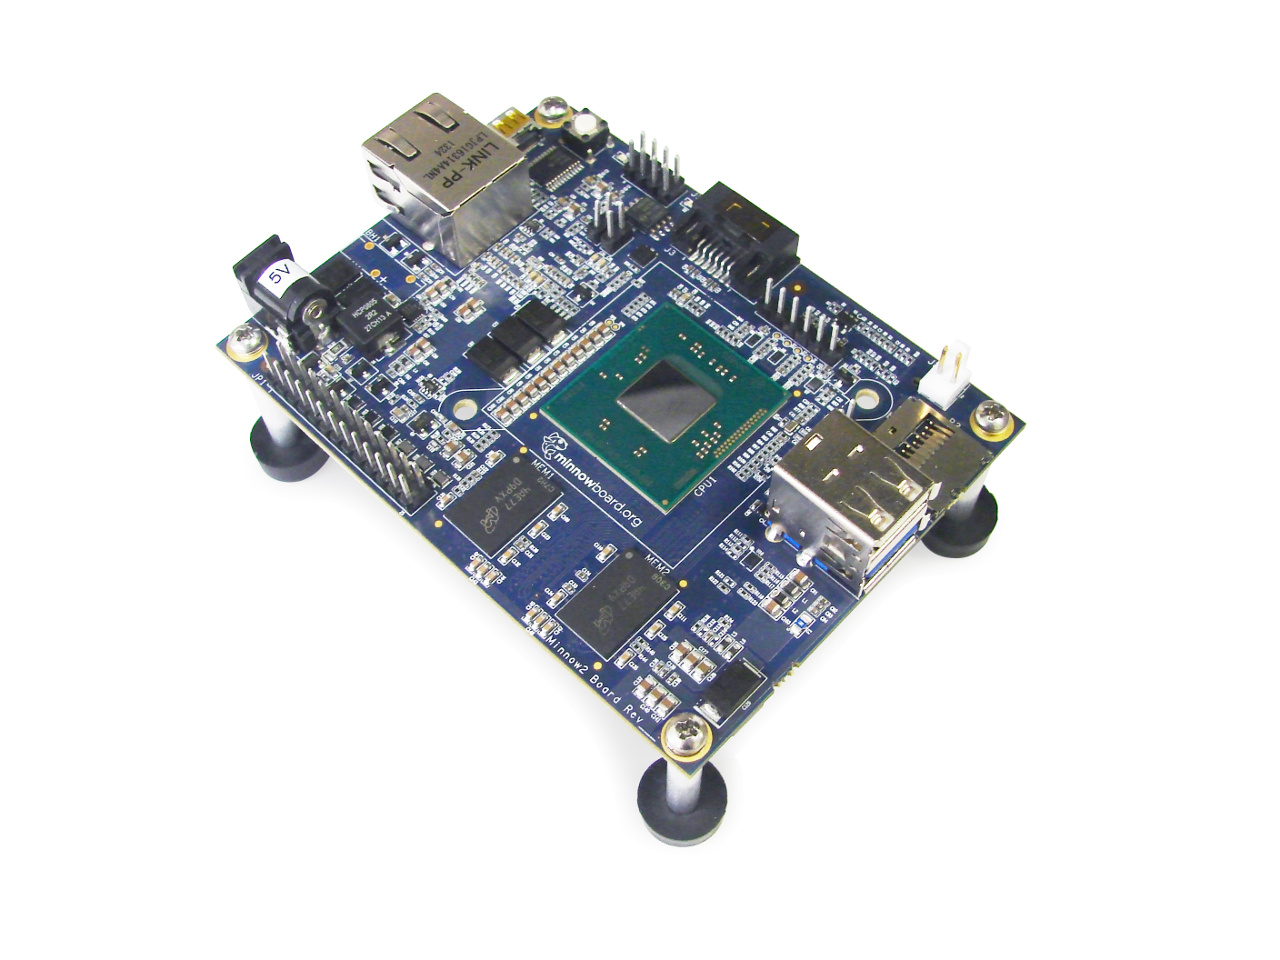
\includegraphics[width=0.75\textwidth]{images/minnow-max.jpg}.png
\caption{The Minnow board Max}
\label{fig:4.1}
\end{figure}


\begin{figure}[H]
\centering
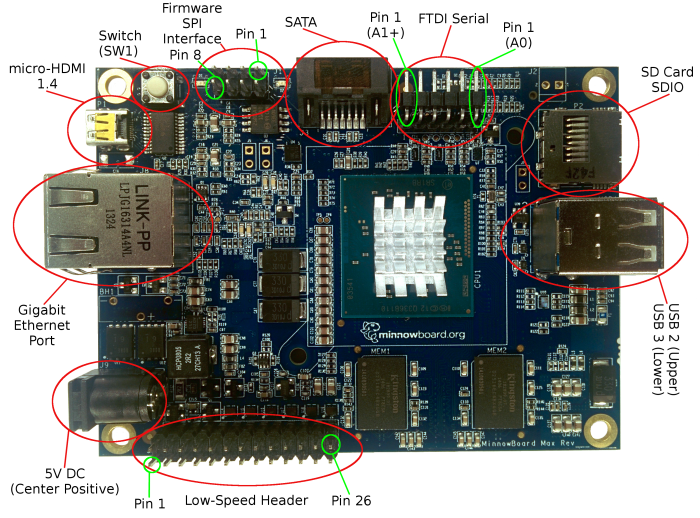
\includegraphics[width=0.75\textwidth]{images/minnow-max-2.png}
\caption{Connection Ports of the Minnow board Max}
\label{fig:4.2}
\end{figure}

\subsection{Embedded Operating System} 

Typical embedded system often does not contain an operating system.  In order
to perform the experiments we need a full Operating System running on the
development board. This means that it will require a boot manager, a full file
system , kernel and user space.  As we can see in \cite{minnowboard} the board
support multiple kind of Operating Systems. The OS we are going to test are : 

\begin{itemize}
    \item Fedora project (Linux base) \cite{fedora}
    \item Clear Linux for Intel Architecture (Linux base) \cite{clear-linux}
    \item Yocto project (Linux base) \cite{yocto-project}
\end{itemize}

We will need to experiment which one is better for our needs. The reason why to
prove multiple  operating systems is because is necessary to find the best one.
There are multiple configurations inside each one that make the performance of
the distributed system change. 

\subsection{Embedded Firmware}

The Minnow Board MAX platform is a low cost, commercially available, reference
platform for hardware, software and firmware developers who wish to work within
an open design development environment. Minnow Board MAX design specifications
and materials have been provided to the open community for the purpose of
enabling the community to experiment and develop technical solutions based upon
the Minnow Board MAX design.

The Minnow Board MAX firmware download page presents firmware components for the
Minnow Board MAX reference board. This firmware is provided to the community for
the purpose of enabling open development and experimentation. For this
experiment we have download the official BIOS Firmware Binary Images
\cite{minnowmax-firmware}


\section{Message-passing library interface}
\noindent

MPI (Message-Passing Interface) is a message-passing library interface
specification. MPI addresses primarily the message-passing parallel programming
model, in which data is moved from the address space of one process to that of
another process through cooperative operations on each process

MPI is not a language, and all MPI operations are expressed as functions,
subroutines, or methods, according to the appropriate language bindings which,
for C and FORTRAN, are part of the MPI standard. The standard has been defined
through an open process by a community of parallel computing vendors, computer
scientists, and application developers

Despite all the advantages that MPI has it is not widely used in embedded
systems (due to the fact that these abstraction layers require extensive
system resources with comprehensive operating systems support, which may not be
available to an embedded platform) but as we have seen this is now possible. We
do have a powerful ultra-low-voltage microprocessor platform
\cite{minnowboard} and we do have robust distributed operating systems running on
those platforms. The missing part now is to set up the message passing library
interface on the top of all the system. 

Recent researches \cite{Saldana} \cite{Gallego} \cite{McMahon} describe
proof-of-concept MPI implementations targeting embedded systems, showing an
increasing interest in the topic. However none of theme has been implemented in
the current embedded Linux operating systems (like the ones generated with
Yocto project\cite{yocto-project}) nor the standard Linux (like
Fedora\cite{fedora})

After a quick review on the current operating systems we found that the only
one missing the MPI implementation was actually the Yocto project.


\begin{center}
\begin{tabular}{ | l | r |}
    \hline
    Operating System & MPI library  \\ \hline
    Fedoras & Implemented  \\ \hline
    Clear Linux for Intel Architecture & Implemented  \\ \hline
    OS generated with Yocto project & Not Implemented  \\ \hline
\end{tabular}
\captionof{table}{MPI implementation in Linux OS supported by Minnow board}
\label{tab:4.2}
\end{center}

Because of that on of the experiment was the implementation of the MPI library
in the Yocto project. 

\section{MPI Benchmarks}
\noindent

The benchmarks we are going to run are the MPI bench version 4
\cite{mpibench}.This is a program to measure the performance of some critical
MPI functions. By critical we mean that the behavior of these functions can
dominate the run time of a distributed application.

MP Bench currently tests eight different MPI calls. The following functions are
measured:

\begin{itemize}
    \item Bandwidth (BB/second)
    \item Gap Time (time to launch a message and continue) (Us)
    \item Roundtrip or 2 * Latency (transactions/second)
    \item Asynchronous Bidirectional bandwidth (KB/second)
    \item Broadcast (KB/second)
    \item Sum reduction (KB/second)
    \item All-reduce (KB/second)
    \item AlltoAll (KB/second)
\end{itemize}



All tests are timed in the following manner.

\begin{itemize}
    \item Set up the test.
    \item Start the timer.
    \item Loop of operations over the message size as a power of two and the
iteration count.
    \item Verify that those operations have completed.
    \item Stop the timer.
    \item Compute the appropriate metric
\end{itemize}

By default, MP-Bench measures messages from 4 bytes to 216 bytes, in powers of
two for 100 iterations. Each test is run a single time before testing to allow
for cache setup and routing. The cache is then flushed before each repetition
and before each new message size is tested. The cache is not flushed however
between iterations on the same message size, which are averaged

For simplicity purposes, we will refer to two different types of tasks in
MPBench, the master of which there is only one, and the slaves of which their
may be any number. The point-to-point tests only use two tasks, a master and a
slave. The other tests run with any number of slaves, the default being
sixteen.

We will describe each one of the tests in order to understand the experiments.


\subsection{Bandwidth}

MPBench measures bandwidth with a doubly nested loop. The outer loop varies the
mes-sage size, and the inner loop measures the send operation over the
iteration count. After the iteration count is reached, the slave process
acknowledges the data it has received by sending a four byte message back to
the master. This informs the sender when the slaves have completely finished
receiving their data and are ready to proceed. This is necessary, because the
send on the master may complete before the matching receive does on the slave.
This exchange does introduce additional overhead, but given a large iteration
count, its effect is minimal.

The master's pseudo code for this test is as follows:

\begin{lstlisting}[frame=single,numbers=left]
do over all message sizes 
    start timer
    do over iteration count 
        send(message size) 
        recv (4)
    stop timer
\end{lstlisting}

The slaves' pseudo code is as follows:

\begin{lstlisting}[frame=single,numbers=left]
do over all message sizes 
    start timer
    do over iteration count 
        recv(message size) 
        send(4)
    stop timer
\end{lstlisting}

\subsection{Bidirectional Bandwidth}

MPBench measures bidirectional bandwidth with a doubly nested loop. The outer
loop varies the message size, and the inner loop measures the send operation
over the iteration count. Both processes execute a non-blocking receive, then a
non-blocking send, and then a wait for each iteration. The next iteration is
prevented from proceeding until the previous one is finished by the MPLWaitall0
call, which will not allow execution to continue until both messages have been
completed.

The code for this test is as follows:
 
\begin{lstlisting}[frame=single,numbers=left]
 do over all message sizes
    start timer
    do over iteration count
        immediate (nonblocking) receive(message size)
        immediate (nonblocking) send(message size)
        wait until messages on both ends have been received
    stop timer
\end{lstlisting}


\subsection{Roundtrip}

Roundtrip times are measured in much the same way as bandwidth, except that,
the slave process, after receiving the message, echoes it back to the master.
This benchmark is often referred to as ping-pong. Here our metric is
transactions per second, which is a common metric for database and server
applications. No acknowledgment is needed with this test as it is implicit
given its semantics.

The master's pseudo code for this test is as follows:

\begin{lstlisting}[frame=single,numbers=left]
  do over all message sizes 
    start timer
    do over iteration count
        send(message size)
        recv(message size) 
        stop timer
\end{lstlisting}

The slaves' pseudo code is as follows:

\begin{lstlisting}[frame=single,numbers=left]
do over all message sizes 
    start timer
    do over iteration count
        recv(message size)
        send(message size)
    stop timer
\end{lstlisting}

\subsection{Application Latency}

Application latency is something relatively unique to MPBench. This benchmark
can prop-early be described as one that measures the time for an application
to issue a send and continue computing. The results for this test vary
greatly given how the message passing layer is implemented. For example, PVM
will buffer all messages for transmission, regardless of whether or not the
remote node is ready to receive the data. MPI on the other hand, will not
buffer messages over a certain size, and thus will block until the remote
process has executed some form of a receive. This benchmark is the same as
bandwidth except that we do not acknowledge the data and we report our
results in units of time.

The master's pseudo code for this test is as follows:

\begin{lstlisting}[frame=single,numbers=left]
do over all message sizes 
    start timer
    do over iteration count 
        send(message size) 
    stop timer
\end{lstlisting}    

The slaves' pseudo code is as follows:

\begin{lstlisting}[frame=single,numbers=left]
   do over all message sizes 
        start timer
        do over iteration count 
            recv(message size) 
        stop timer
\end{lstlisting}

\subsection{Broadcast and Reduce}

The two functions are also very heavily used in many parallel applications.
Essentially these operations are mirror images of one another, the different
being that reduce reveres the di-rection of communication and performs some
computation with the data during intermediate steps. Both of these
benchmarks return the number of megabytes per second computed from the
iteration count and the length argument given to function call.

Here is the pseudo code for both the master and the slave:


\begin{lstlisting}[frame=single,numbers=left]
   do over all message sizes 
        start timer
        do over iteration count
            reduce or broadcast(message size)
        stop timer
\end{lstlisting}

\subsection{AllReduce}

AllReduce is a derivative of an all-to-all communication, where every
process has data for every other. While this operation could easily be
implemented with a reduce followed by a broadcast, that would be highly
inefficient for large message sizes. The PVM version of this test does this
exactly, plus an additional barrier call. The goal of including this
benchmark is to spot poor implementations so that the application engineer
might be able to restructure his communication.

Here is the pseudo code for both the master and the slave:

\begin{lstlisting}[frame=single,numbers=left]
    do over all message sizes 
        start timer
        do over iteration count 
            allreduce(message size) 
        stop timer
\end{lstlisting}


\subsection{All-to-all}

MPBench measures a kind of round-robin communication among multiple
processes. The outer loop varies the message size, and the inner loop
measures the send operation over the iteration count. Each process sends a
message of the size of the total message size divided by the number of
processes to every other process.

The code for this test is as follows:

\begin{lstlisting}[frame=single,numbers=left]
    do over all message sizes 
        start timer
        do over iteration count 
            all-to-all(message size)
        stop timer
\end{lstlisting}

\section{Topologies}

In computer networking, topology refers to the layout of connected devices. This
article introduces the standard topologies of networking

Think of a topology as a network's virtual shape or structure. This shape does
not necessarily correspond to the actual physical layout of the devices on the
network. For example, the computers on a home network may be arranged in a
circle in a family room, but it would be highly unlikely to find a ring
topology there.

Network topologies are categorized into the following basic types:

\begin{itemize}
    \item bus
    \item ring
    \item star
    \item tree
    \item mesh
\end{itemize}

More complex networks can be built as hybrids of two or more of the above basic
topologies.

For our experiments we will use the star topology (figure~\ref{fig:4.3}). In
local area networks with a star topology, each network host is connected to a
central hub with a point-to-point connection. So it can be said that every
computer is indirectly connected to every other node with the help of the hub.
In Star topology every node (computer workstation or any other peripheral) is
connected to a central node called hub, router or switch. The switch is the
server and the peripherals are the clients. The network does not necessarily
have to resemble a star to be classified as a star network, but all of the
nodes on the network must be connected to one central device. All traffic that
traverses the network passes through the central hub. The hub acts as a signal
repeater. The star topology is considered the easiest topology to design and
implement. An advantage of the star topology is the simplicity of adding
additional nodes. The primary disadvantage of the star topology is that the hub
represents a single point of failure.

\begin{figure}[H]
\centering
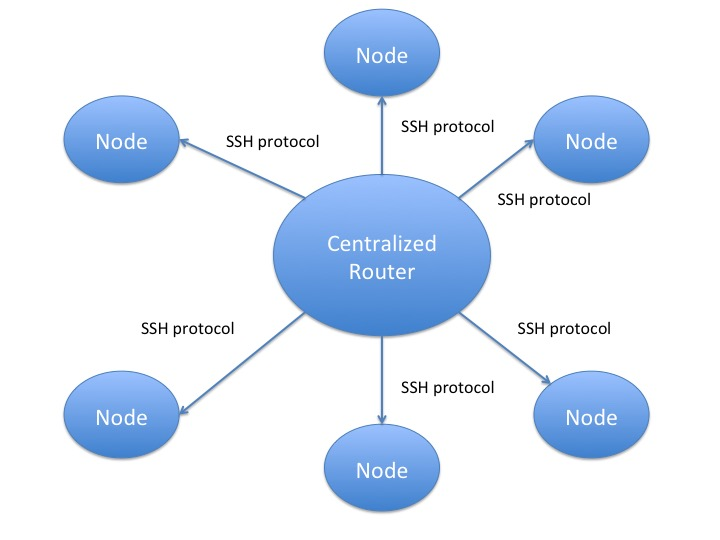
\includegraphics[width=0.75\textwidth]{images/star_topology.png}
\caption{Star topology diagram}
\label{fig:4.3}
\end{figure}


\section{Architecture Diagram}

After understanding all the parts of the system now we can describe the full
architecture of our experiments. The figure~\ref{fig:4.4} shows the diagram of
the final architecture in an star topology. As you can see the system can
increase the numbers of nodes (Minnow board platforms) if we want to increase
the compute capacity.


\begin{figure}[H]
\centering
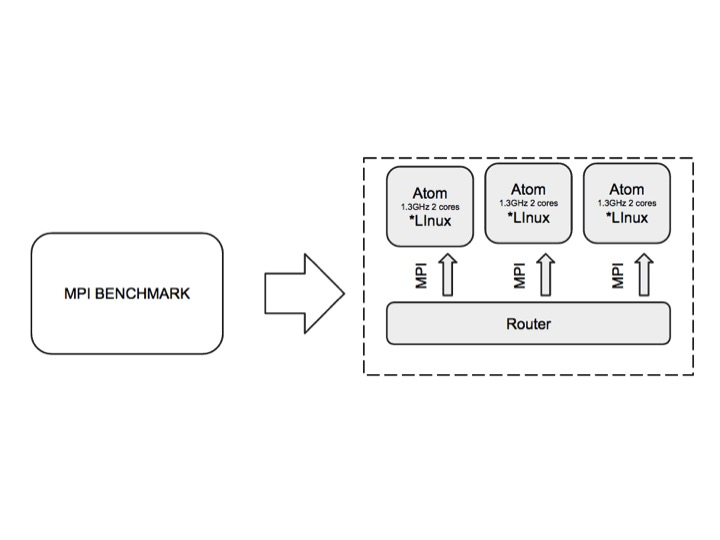
\includegraphics[width=0.75\textwidth]{images/full_diagram.jpg}
\caption{System Architecture Diagram }
\label{fig:4.4}
\end{figure}

\noindent

\clearpage
